\chapter{Ergänzungen zur Laufzeitanalyse von Parsivald}

\section{Workerdichte}

\todoline{Text}

\begin{figure}[!hp]
  
  \captionsetup[subfigure]{singlelinecheck=false}
  \def\subfigwidth{7cm}
  \begin{subfigure}[t]{\subfigwidth}
    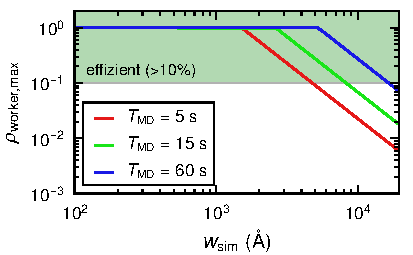
\includegraphics[width=\textwidth]{densitybymdtime}
  \end{subfigure}
  \hfill
  \begin{subfigure}[t]{\subfigwidth}
    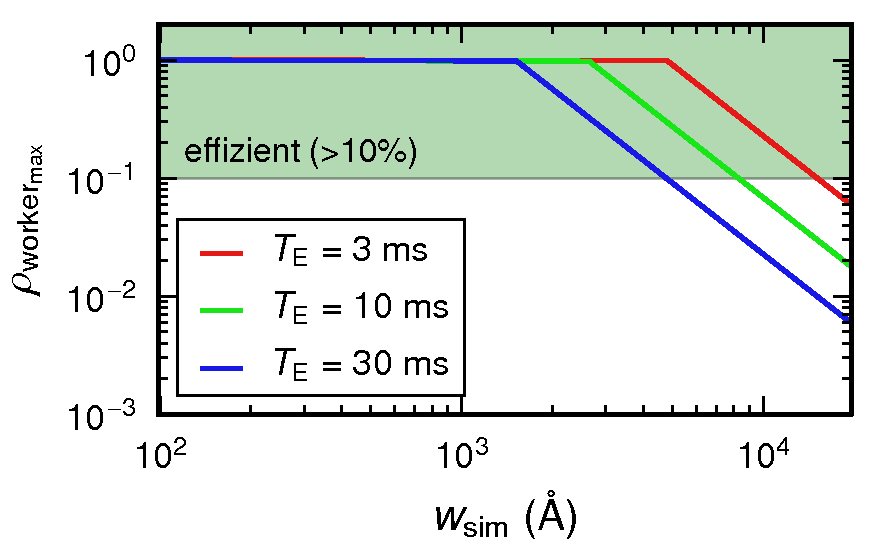
\includegraphics[width=\textwidth]{densitybykmctime}
  \end{subfigure}

  \caption{Abhängigkeiten der maximalen Workerdichte $\rho_{\text{worker}_\text{max}}$}

\end{figure}

\section{Maximale Raumgröße für effiziente Simulationen}
\todoline{Text}

\begin{figure}[!hp]
  \captionsetup[subfigure]{singlelinecheck=false}
  \def\subfigwidth{7cm}
  \begin{subfigure}[t]{\subfigwidth}
    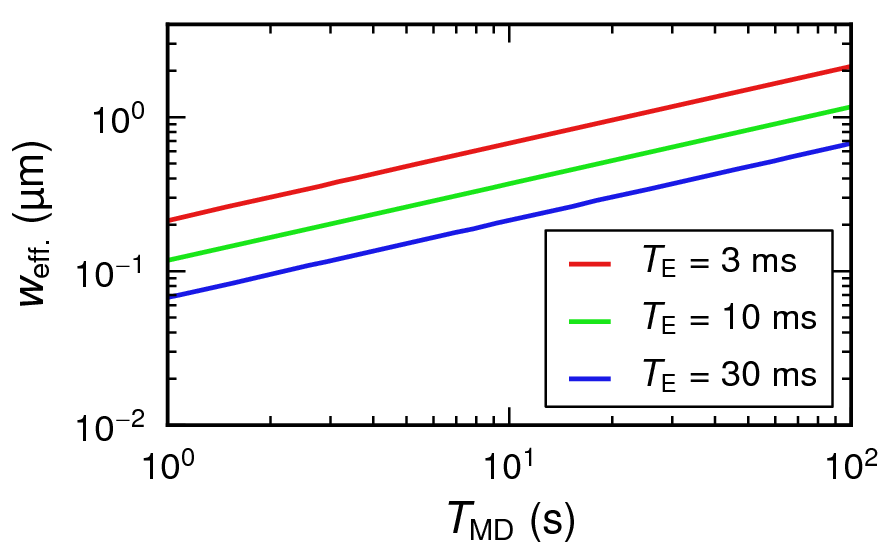
\includegraphics[width=\textwidth]{maxsizebymdtime}
  \end{subfigure}
  \hfill
  \begin{subfigure}[t]{\subfigwidth}
    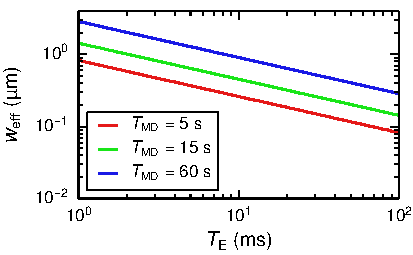
\includegraphics[width=\textwidth]{maxsizebykmctime}
  \end{subfigure}

  \caption{Abhängigkeiten des Maximums der Breite des Simulationsraumes für effiziente Simulationen  $w_{\text{sim}_\text{eff}}$}
  
\end{figure}

\section{Maximale Anzahl paralleler Prozesse}

\todoline{Text}

\begin{figure}[!hp]
  
  \captionsetup[subfigure]{singlelinecheck=false}
  \def\subfigwidth{7cm}
  \begin{subfigure}[t]{\subfigwidth}
    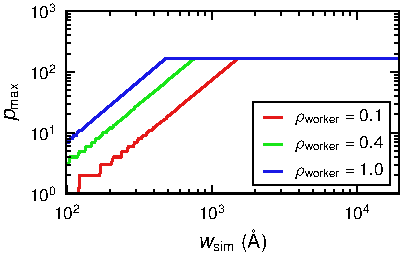
\includegraphics[width=\textwidth]{workersbydensity}
  \end{subfigure}
  \hfill
  \begin{subfigure}[t]{\subfigwidth}
    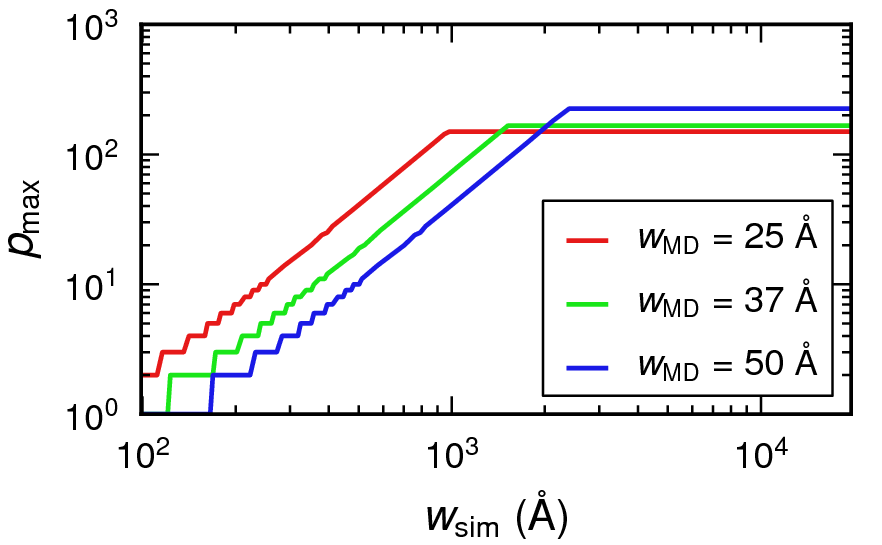
\includegraphics[width=\textwidth]{workersbymdsize}
  \end{subfigure}

  \begin{subfigure}[t]{\subfigwidth}
    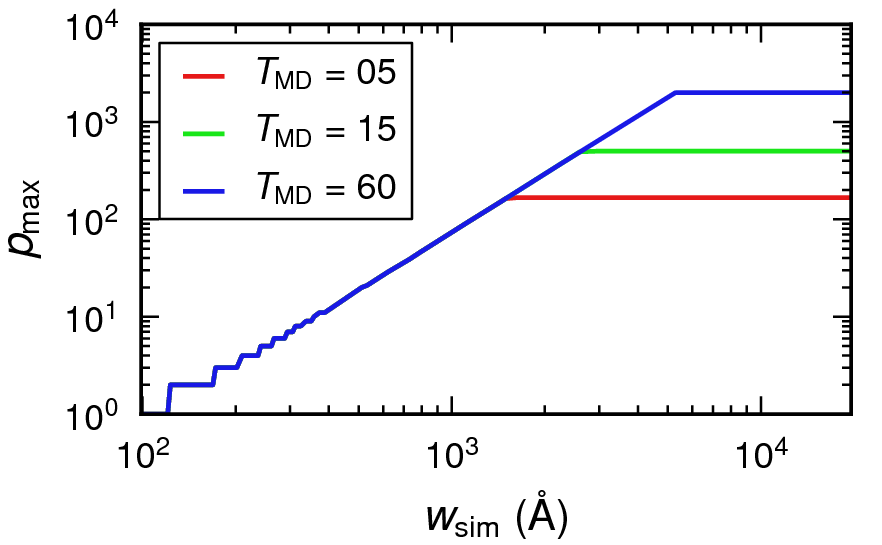
\includegraphics[width=\textwidth]{workersbymdtime}
  \end{subfigure}
  \hfill
  \begin{subfigure}[t]{\subfigwidth}
    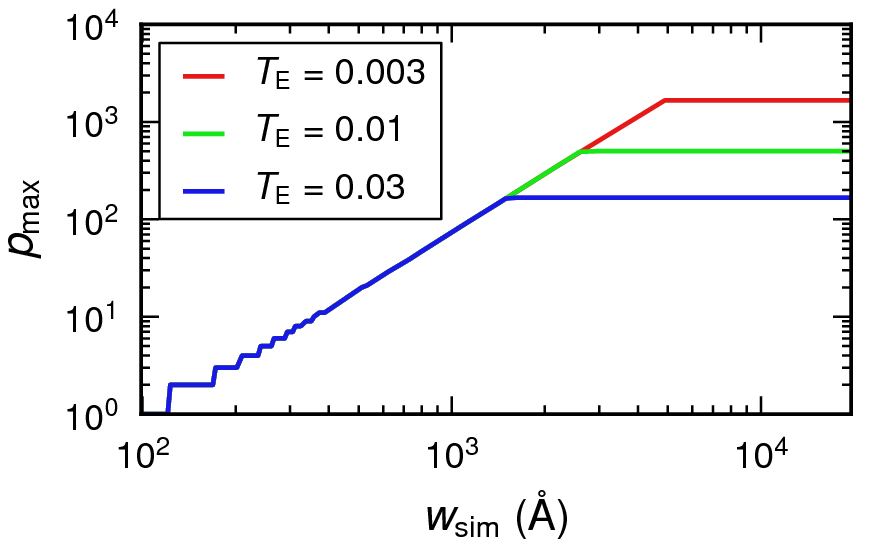
\includegraphics[width=\textwidth]{workersbykmctime}
  \end{subfigure}
  \hfill

  \caption{Abhängigkeiten der maximalen Zahl paralleler Prozesse}
  
\end{figure}


\section{Minimale Laufzeit}

\todoline{Text}

\begin{figure}[!hp]
  
  \captionsetup[subfigure]{singlelinecheck=false}
  \def\subfigwidth{7cm}
  \begin{subfigure}[t]{\subfigwidth}
    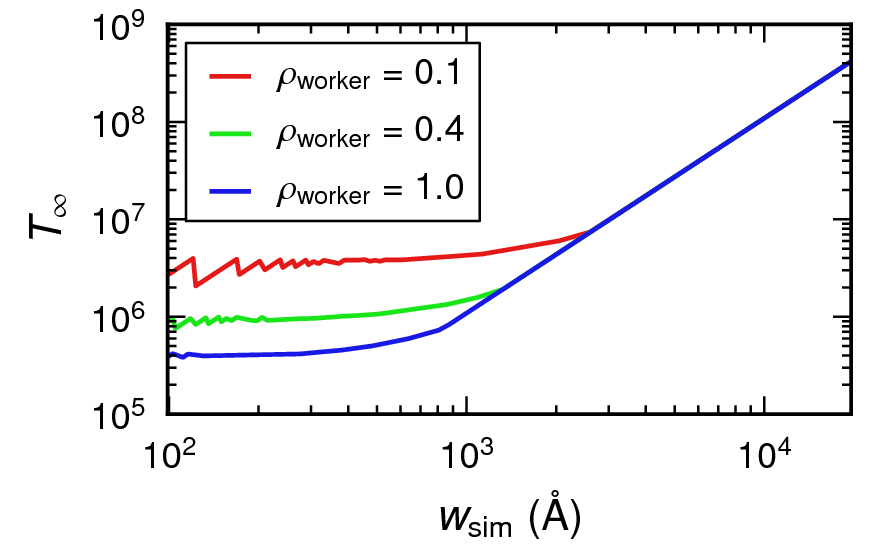
\includegraphics[width=\textwidth]{runtimebydensity}
  \end{subfigure}
  \hfill
  \begin{subfigure}[t]{\subfigwidth}
    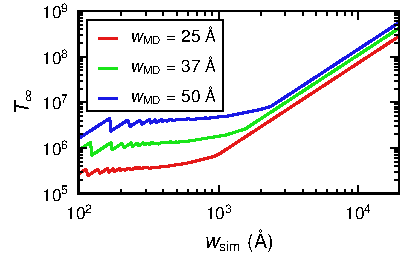
\includegraphics[width=\textwidth]{runtimebymdsize}
  \end{subfigure}

  \begin{subfigure}[t]{\subfigwidth}
    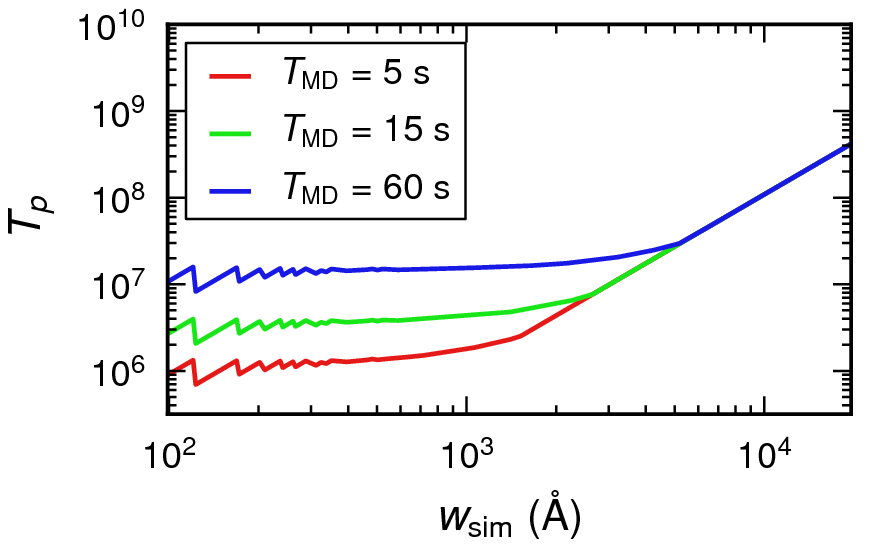
\includegraphics[width=\textwidth]{runtimebymdtime}
  \end{subfigure}
  \hfill
  \begin{subfigure}[t]{\subfigwidth}
    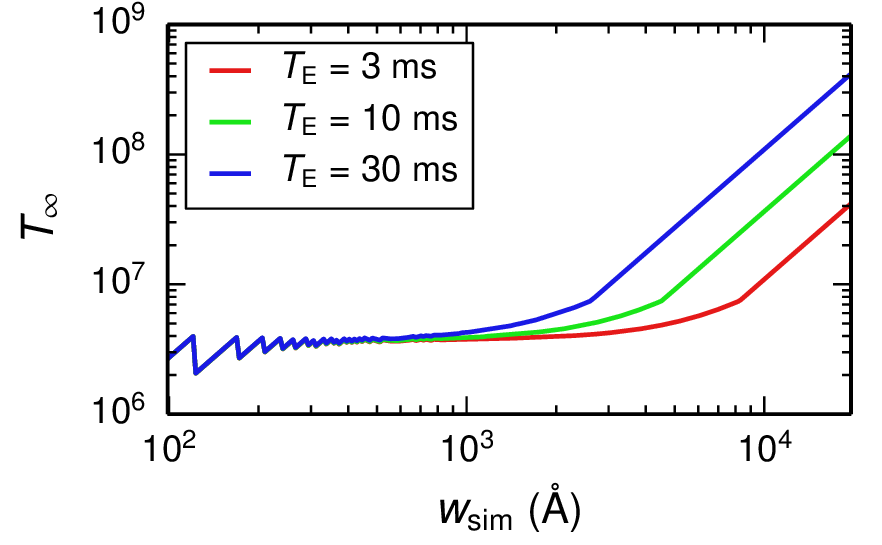
\includegraphics[width=\textwidth]{runtimebykmctime}
  \end{subfigure}
  \hfill

  \caption{Abhängigkeiten der Laufzeit}
  
\end{figure}
